\chapter[Pattern and Scale in Ecology and Earth Observations]{Pattern and Scale in Ecology and Earth Observations Science}

Christopher B. Anderson

\section{Abstract}

Human activity and land-use change are dramatically altering the sizes, geographical distributions and functioning of biological populations worldwide, with tremendous consequences for human well-being. Yet our ability to measure, monitor and forecast biodiversity change–crucial to addressing it—remains limited. Biodiversity monitoring systems are being developed to improve this capacity by deriving metrics of change from an array of \textit{in situ} data (e.g. field plots or species occurrence records) and Earth observations (EO; e.g. satellite or airborne imagery). However, there are few ecologically based frameworks for integrating these data into meaningful metrics of biodiversity change. Here, I describe how concepts of pattern and scale in ecology could be used to design such a framework. I review three core topics: the role of scale in measuring and modelling biodiversity patterns with EO, scale-dependent challenges linking \textit{in situ} and EO data and opportunities to apply concepts of pattern and scale to EO to improve biodiversity mapping. From this analysis emerges an actionable approach for measuring, monitoring and forecasting biodiversity change, highlighting opportunities to establish EO as the backbone of global-scale, science-driven conservation.

\section{Introduction}

Global biodiversity monitoring is a crucial but challenging task, as human activities are changing the structure and composition of biological populations at all taxonomic levels \cite{Dirzo2014-wd,Ceballos2017-un}. Mitigating biodiversity loss will require understanding the rates, magnitudes and geography of these changes \cite{Laurance2012-ic, Mendenhall2014-fh}. However, considering the scope of action required for mitigation, our knowledge of global biodiversity change remains limited \cite{Daily1999-mv,Pereira2012-vm}. Furthermore, what is known about biodiversity change is complicated by taxonomic, geographical and recency biases \cite{Boakes2010-xq,Donaldson2016-er,Gonzalez2016-gh}.

Novel biodiversity monitoring systems are being developed to overcome these biases by systematically assessing change for multiple taxa over large extents \cite{Scholes2008-ta,Scholes2012-ec,Fernandez2015-na}. To support these systems, several groups have developed novel approaches to monitor species, communities and ecosystems over time using globally consistent metrics of change \cite{Butchart2010-we, Jetz2012-mw, Metzger2013-mz, Pereira2013-pk}. These metrics are biological, sensitive to change, and ecosystem agnostic, enabling consistent monitoring protocols worldwide \cite{Geo_bon2017-ak}. These efforts have been greatly bolstered by increasing access to globally available \textit{in situ} biodiversity observations \cite{Geijzendorffer2016-xv, Culina2018-ih}. However, as \textit{in situ} data alone are often insufficient for assessing global diversity patterns (\textit{sensu} the Linnean and Wallacean shortfalls \cite{Bini2006-an, Brito2010-gs}), researchers have looked for complementary data to support monitoring efforts.

Earth observations (EO; e.g. satellite or airborne imagery) complement \textit{in situ} data by providing repeat, thematically consistent and spatially continuous measurements of terrestrial ecosystems, characterising biodiversity patterns over large, undersampled areas. However, linking fine-scale field and EO data faces many challenges, including incomplete sampling efforts (i.e., where field measurements do not adequately characterise the extent of environmental variation; \cite{Marvin2014-ms}) and reconciling scale mismatches (e.g., where field plots are much smaller than EO measurements). Developing EO‐based biodiversity monitoring systems will require a comprehensive approach to link these data \cite{Turner2014-kq,Pettorelli2016-wi}.

Scale plays a key role in both ecology and EO science, and identifying shared scaling dynamics could provide a basis for bridging these disciplines. Understanding the roles of spatial and temporal scales in biological communities is a central topic in ecology, and is referred to as the problem of pattern and scale \cite{Wiens1989-yi,Levin1992-ga}. The problem of pattern and scale emphasises that multiple ecological processes often determine the spatial distributions of biodiversity patterns, and that these processes can act across multiple spatial and organismal scales \cite{Withers1999-ls,Waring2010-cl,Chase2013-gl}. Therefore, there is rarely a single measurement scale that best identifies how specific processes drive patterns \cite{Hutchinson1953-md}. EO measurements are subject to similar scale dependencies: the grain size of an EO sensor often determines which patterns can be measured (Fig. \ref{fig:spatiotemporal}) \cite{Lechner2010-pi,Anderson2012-ql,Nagendra2013-gn}, and multi‐scale EO analyses can reveal the influences of multiple processes driving biodiversity patterns \cite{Keil2012-ad,Taylor2015-ql}. Applying concepts of pattern and scale in ecology to EO could provide a means to better link these fields, paving the way for improved biodiversity monitoring.

Here, I review the scales at which EO have been used to measure and model metrics of biodiversity change, and the role of scale in linking field data with EO. This is not strictly a review of which biodiversity patterns EO can measure (\textit{sensu} \cite{Roughgarden1991-so,Turner2003-dp,Wang2010-ev,Pettorelli2014-yz, Lausch2016-fk}). Instead, this review addresses three questions: 

\begin{enumerate}
    \item At what scales have current and historical EO been used to measure or model spatial biodiversity patterns? 
    \item What are the major challenges linking field‐based and EO‐based biodiversity measurements, and how does scale impact these challenges?
    \item How can concepts of pattern and scale, applied to EO, facilitate the translation of biodiversity patterns across scales? 
\end{enumerate}

\section{Components of Pattern and Scale in Ecology}

\begin{figure}[!ht]
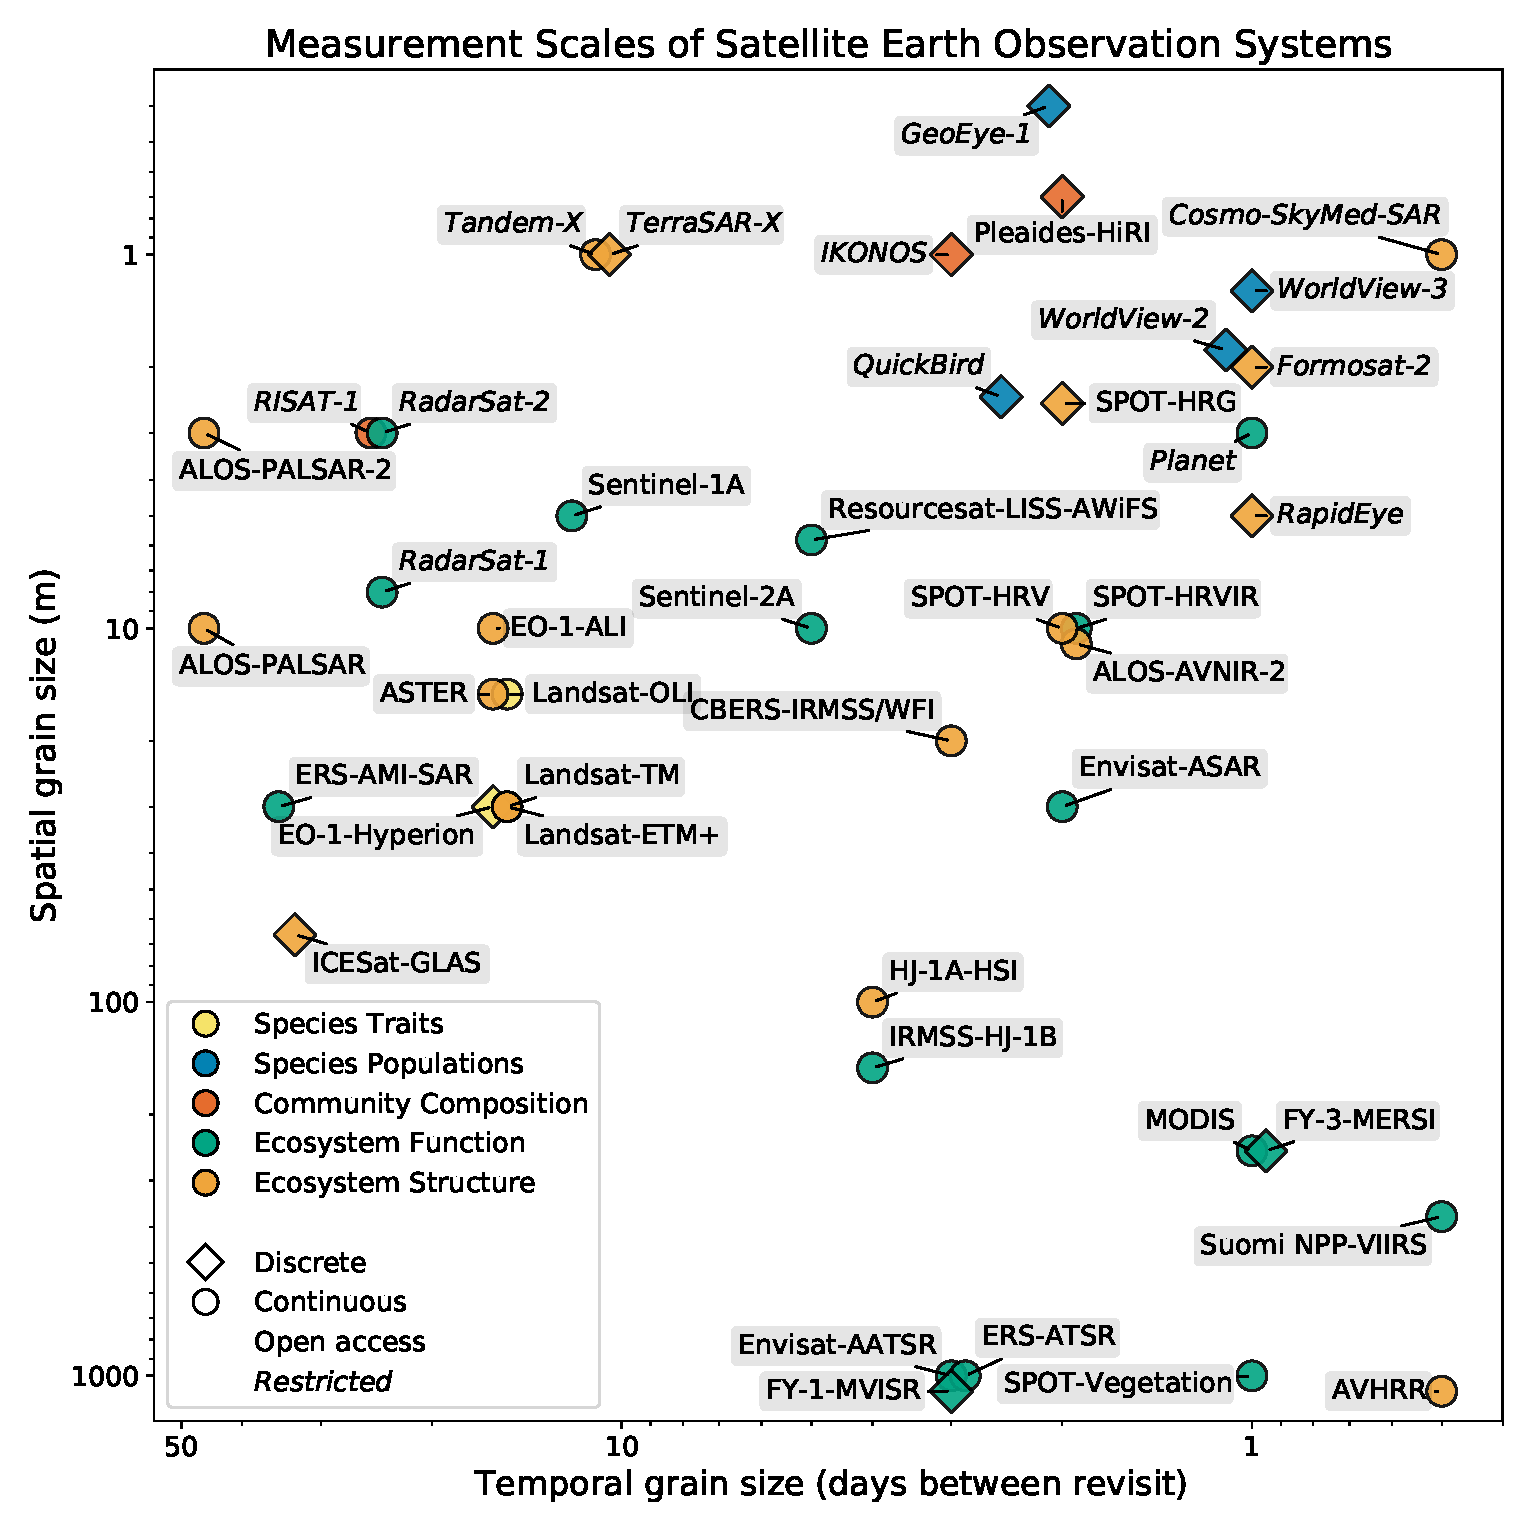
\includegraphics[width=\textwidth]{ch1-spatiotemporal}
\centering
\caption[Spatial and temporal and grain sizes for 44 current and historic satellite Earth observation (EO) sensors.]{Spatial and temporal and grain sizes for 44 current and historic satellite Earth observation (EO) sensors, colored by EBV class. Several sensors have been used to measure multiple biodiversity patterns, and the most cited or most novel were selected in these cases.}
\label{fig:spatiotemporal}
\end{figure}

Explorations of pattern and scale in ecology focus on two distinct but related measurement scales: grain size and extent. In this review, I refer to these scales in a spatial sense, though temporal grain size could describe the frequency of observations (e.g., one diurnal cycle for net primary productivity) and temporal extent could describe the total time over which an ecological process occurs (e.g. phenological variation throughout a year). Furthermore, I adopt the classes and metrics of biodiversity change from the Essential Biodiversity Variables framework \cite{Pereira2013-pk}, and refer to these metrics as biodiversity patterns. This framework captures the multiple biological scales of diversity (i.e., variation in genes, species, communities and ecosystems) as opposed to a more narrow interpretation that refers to biodiversity as variations in species richness, abundance and evenness. I believe these disaggregated classes and metrics more comprehensively address the patterns that can be measured and modelled using EO. In this section I discuss how concepts of pattern and scale in ecology apply in biodiversity and EO contexts, then I review domains of scale, which constrain efforts to generalise patterns across scales. See the \textit{Glossary} for clarifications on the terms and acronyms used.

\subsection{Changing Measurement Scales}

Measurement scales are often selected to understand biodiversity patterns or ecological processes in a specific region, or for a specific species, population or ecosystem. A key scaling dynamic is that when the scale of measurement changes, the variation within that measurement is also subject to change \cite{Wiens1989-yi,Levin1992-ga}. For example, early biodiversity/ecosystem function research suggested the relationship between species richness and productivity to be unimodal, predicting peak biomass accumulation at intermediate diversity for both primary and secondary productivity \cite{Rosenzweig1993-mo}. However, this functional form was shown to be an artefact of plot size as opposed to any ecological process \cite{Oksanen1996-bx}, and a global synthesis found mixed evidence for a generalised relationship in any form \cite{Adler2011-zc}. Recently, however, long‐term studies addressing scale directly have demonstrated a positive yet saturating diversity‐productivity relationship across multiple ecosystem \cite{Liang2016-dv,Hungate2017-ax}.

Measurements of community‐scale patterns, like species richness and turnover (i.e. $\alpha$ and $\beta$ diversity), have also been shown to vary directly with scale \cite{Rosenzweig1995-hc}. Coarse grains are expected to contain higher species richness per grain, and thus lower species turnover between grains \cite{Nekola1999-ks,Whittaker2001-lw}. This is because larger grains are expected to contain more rare species and more environmental variation (e.g. more variation in niche space; \cite{Keil2015-nl}. Indeed, \cite{Hurlbert2007-dc} showed systematic increases in species richness at coarser grain sizes for birds in South Africa and Australia. Similarly, species turnover has been shown to decrease at coarser grains for birds in Britain and North America \cite{Mac_Nally2004-ly,Gaston2007-yf}, and for mammals in Mexico \cite{Arita2002-jk}.

Measurement scales likewise determine which biodiversity patterns can be measured by EO (Fig. \ref{fig:spatiotemporal}). Satellite EO have historically focused on measuring ecosystem‐scale patterns, due to the coarse grain sizes of historic sensors. Coarse grain EO sensors measure ecosystem‐scale patterns, like disturbance regime \cite{Wang2012-bo, Kogan2015-mz} and ecosystem extent \cite{Maillard2008-dk, Bartsch2009-ze}. Fine‐grain sensors measure species‐ and community‐scale patterns like species occurrences \cite{Immitzer2012-no} and taxonomic diversity \cite{Khare2018-dx}. Measuring species traits has likewise proven challenging due to difficulties distinguishing individual organisms in EO imagery \cite{Nagendra2013-gn, Jetz2016-bx}. But some plant traits, like canopy nitrogen content and photosynthetic rates, can be retrieved even at moderate grain sizes \cite{Martin2008-te,Serbin2014-ta}. High frequency measurements can map temporally sensitive processes like vegetation phenology \cite{Bradley2007-dt}, but high frequency, continuous measurements often come at the expense of coarser grain sizes. Fortunately, an increasing number of fine‐grain EO sensors now in orbit is enabling EO biodiversity mappers to focus on more species‐ and community‐scale patterns (Fig. \ref{fig:timeline}) \cite{Butler2014-tp}.

There are key similarities in scaling dynamics between field and EO data: grain size and extent both constrain within and between‐grain measurement variation. Large field plots tend to contain more species per plot, and lower turnover between plots. Likewise, large EO pixels tend to contain more organisms per grain, and lower turnover between grains. This constrains measurement specificity. However, the grain size of an EO sensor only constrains the smallest unit of measurement; these data can be spatially aggregated to larger scales \cite{fisher1997pixel}. For example contiguous pixels measuring the same tree could be aggregated to delineate a single crown, or clusters of forested pixels could be aggregated to delineate forest fragments \cite{Yao2015-dp}. This enables comparisons between crowns or across fragments, instead of pixels, helping bridge the gap between spatial and biological scales. This is known as object‐based image analysis \cite{blaschke2008object}, which is likely to become more common in biodiversity monitoring as novel segmentation algorithms are tuned for EO \cite{NIPS2012_4824,basu2015deepsat}. And though this approach facilitates ecological interpretations of EO data, there are key scaling dynamics associated with aggregating data across scales.

\subsection{Domains of Scale}

One tenet of the problem of pattern and scale in ecology suggests that, since multiple ecological processes often drive spatial biodiversity patterns, there is rarely a single scale at which any pattern must be examined \cite{Hutchinson1953-md,Levin1992-ga}. These patterns are often examined at multiple points along biological, spatial or temporal scale spectrums in order to understand how multiple processes drive patterns. For example, the drivers of net primary productivity in plants could be examined at leaf, whole plant and landscape scales. The leaf, plant and landscape, here, represent domains of scale: the scales over which patterns either do not change, or change monotonically with changes in scale \cite{Wiens1989-yi}. In this example, fine‐scale processes, like intra-crown shading, may drive the majority of variation in leaf‐scale productivity, but may be less important at landscape scales, where ecosystem processes like resource availability drive the majority of variation \cite{Field1995-jy}. Partitioning biodiversity patterns into genetic, species, community and ecosystem‐scale patterns organises them as domains of scale; the processes that drive variation in species‐scale patterns are expected to drive variation in ecosystem‐scale patterns through separate but potentially nested pathways \cite{Pereira2012-vm,Pereira2013-pk}.

Constraining measurements and models to discrete domains of scale is key for simplifying predictions of how species respond to environmental change \cite{Field1991-pk}. Multi‐scale analyses have been used to identify domains of scale, revealing where transitions across scales has nonlinear effects on observed patterns \cite{Palmer1994-ya}. In community ecology, hierarchical regression models have been employed to this end \cite{Legendre2005-zb}. For example, \cite{Keil2012-ad} tested how $\beta$-diversity patterns for birds, butterflies, plants, amphibians and reptiles across Europe varied with distance, climate and land cover. They found $\beta$-diversity (here, dissimilarity) decreased systematically at coarser grain sizes for each taxon. Their hierarchical analysis found climate was important for predicting $\beta$-diversity patterns at coarse grain sizes, and land cover was important at fine‐grain sizes, though these effects varied by taxon. Their results suggest that efforts to predict changes in turnover should assess the effects of multiple domains of scale simultaneously, and that these scale dependencies are taxon‐specific.

\begin{figure}[!ht]
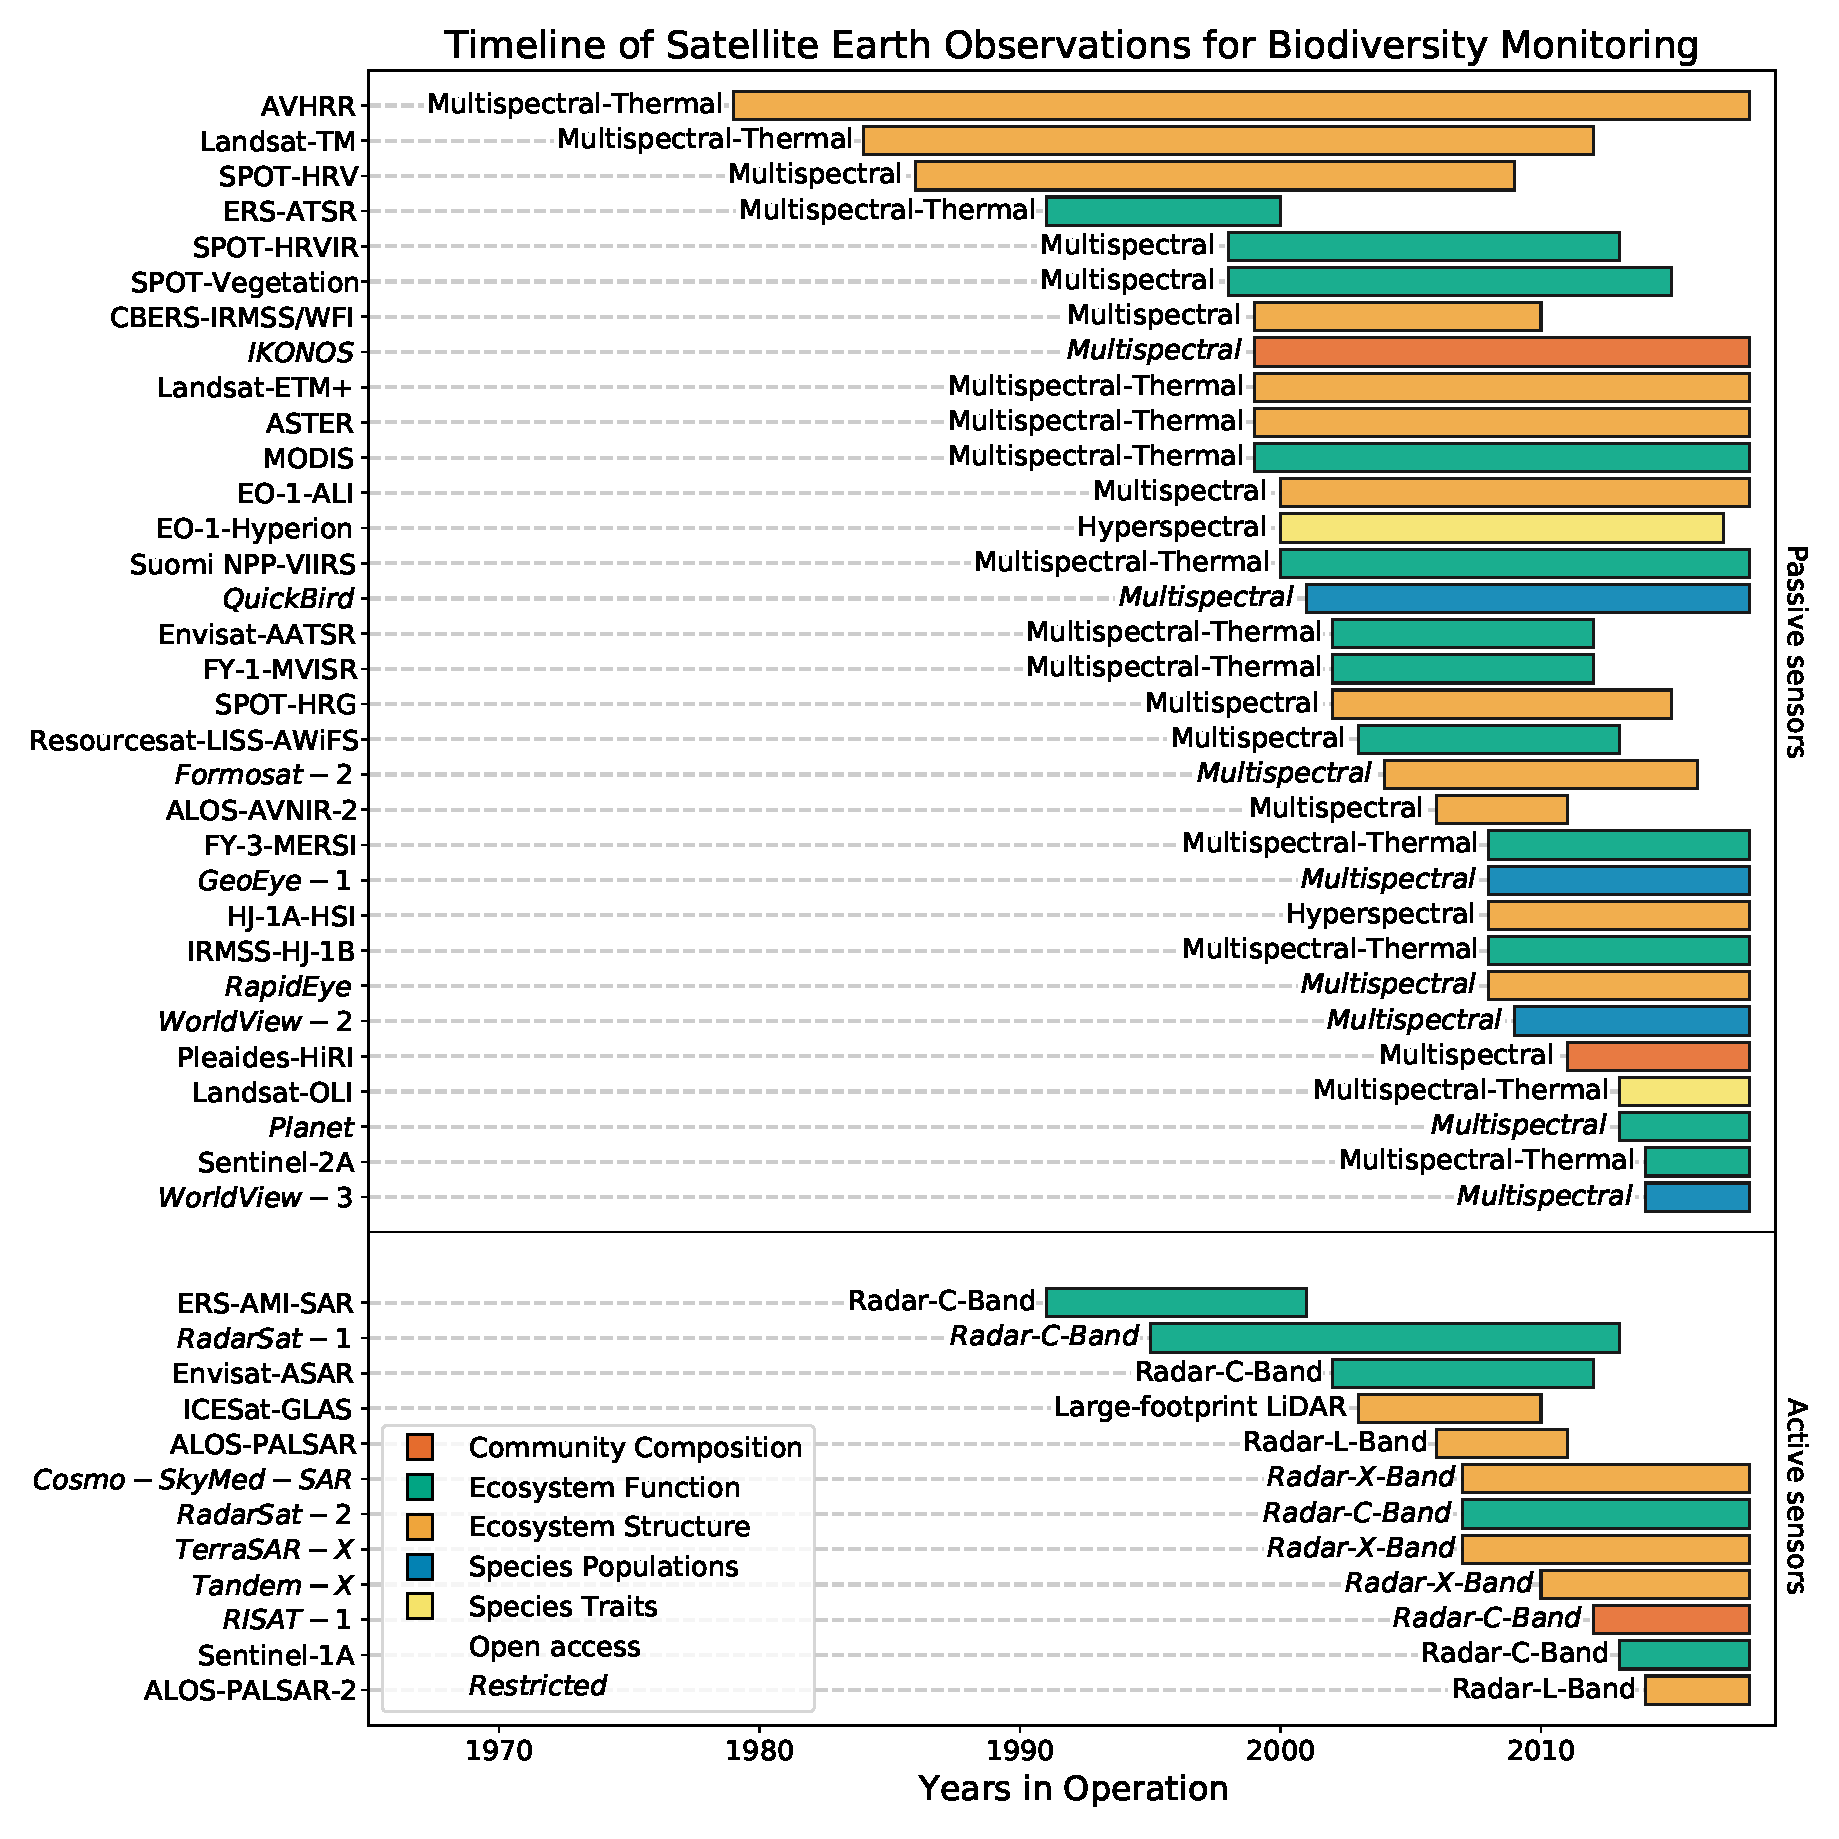
\includegraphics[width=\textwidth]{ch1-timeline}
\centering
\caption[Temporal extents of current and historic satellite sensors.]{Temporal extents of current and historic satellite sensors, colored by EBV class. Temporally coincident measurements can be jointly analyzed in a multi‐sensor fusion framework to increase data dimensionality.}
\label{fig:timeline}
\end{figure}

The domains of scale where processes drive patterns may not always be known \textit{a priori}, however. These are often identified using multi‐scale sensitivity analysis. For example, \cite{Mendenhall2011-mu} developed a multi‐scale model to predict how bird community composition changed with land cover change in Costa Rica. They assessed species turnover along tree cover gradients, finding turnover varied nonlinearly with cover at both fine and coarse grain sizes. Their results suggested there are two domains of scale over which tree cover patterns determine turnover patterns for birds (perhaps tracking habitat and resource availability, respectively; \cite{morrison2012wildlife}). Furthermore, their results suggested tree cover change could serve as a proxy to predict turnover in other communities. Indeed, \cite{Mendenhall2016-xz} found tree cover change predicted changes in composition for understory plants, non‐flying mammals, bats, reptiles and amphibians. Furthermore, they found the grain size of tree cover which best predicted turnover varied by taxon. Their work highlights one approach to mapping biodiversity change with EO – identifying domains of scale through multi‐scale sensitivity analysis, then modelling turnover via regression with EO‐derived environmental features.

\section{Measuring and Modeling Biodiversity Patterns with EO}

There are currently two principal paradigms for mapping biodiversity patterns with EO \cite{Turner2003-dp}. First is to directly measure species, community or ecosystem‐scale patterns. Examples of this paradigm include identifying individual organisms within a species \cite{Gairola2013-fk} or mapping the extent of an ecosystem \cite{Henderson2008-xd}. Second is to model biodiversity patterns indirectly using EO as predictive environmental features. Examples of this paradigm include modelling species richness from measurements of habitat structure \cite{Saatchi2008-jq}, or modelling species distributions and turnover using land cover maps \cite{Guisan2005-kg, Keil2012-ad}. Here I review the roles of measurement type and measurement scales in these paradigms, focusing on biodiversity patterns mapped by current and historic spaceborne sensors that can be accessed by biodiversity monitoring systems (Table \ref{tab:eo-sensors}).

\subsection{Measuring Biodiversity Patterns}

EO measurements of biodiversity patterns are characterised by three key properties: sensor type, sensor fidelity and measurement scales \cite{Pettorelli2014-pn, OConnor2015-bj}. Sensor type determines which patterns can be measured, sensor fidelity constrains the variation in those measurements, and measurement scales determine the amount of variation within and between measurements \cite{Jensen1987-nd}. Passive sensors, such as multispectral sensors and imaging spectrometers, measure patterns of ecosystem function, like leaf area index \cite{Fensholt2004-ew}, vegetation phenology \cite{Fan2015-gg} or disturbance regime \cite{Feng2008-hb}. Active sensors, such as radio or light detection and ranging sensors (i.e., radar and lidar), often measure patterns of ecosystem structure, like tree height \cite{Lefsky2005-nh} and ecosystem extent \cite{Bartsch2009-ze}. These distinctions are not axiomatic; multiple sensor types have been used to measure the same pattern \cite{Pohl1998-ze}. Both radar and multispectral sensors have been used to measure tree cover, for example. Radar sensors map tree cover by measuring woody structural and hydrological characteristics \cite{Walker2010-md, Shimada2014-wi}, and multispectral sensors map tree cover by measuring leaf optical properties like pigment concentrations \cite{Sims2002-ge, Sexton2013-rk}.

Using multiple sensors to map a single biodiversity pattern can improve model accuracy and reduce sensor‐specific uncertainties, and is known as multi‐sensor fusion \cite{Hall1997-ux}. Consider, again, the application for tree cover mapping. Though multispectral sensors are sensitive to pigment concentrations, measuring tree cover in leaf‐off conditions is a challenge; exposed branches are optically similar to dried grass or other non‐photosynthetic vegetation \cite{Asner1998-rw}. Radar is sensitive to woody biomass regardless of phenology. but can itself be noisy due to speckling \cite{lee1994speckle}. To obviate this issue, \cite{Naidoo2016-fp} mapped cover in a South African savannah by combining multispectral and radar measurements. Combined, they mapped tree cover with 90\% accuracy, which was 12\% higher than using either sensor independently. Multi‐sensor fusion approaches to biodiversity mapping hold great promise for reducing sensor‐specific uncertainties, and are poised to become more valuable as access to novel sensor types increases (Fig. \ref{fig:timeline}) \cite{Butler2014-tp, Schulte_to_Buhne2018-ai}.

Comparing measurements from similar sensor types with different grain sizes has been used to assess the importance of scale in measuring biodiversity patterns. For example \cite{Brown2006-pu} compared NDVI measurements from four spaceborne multispectral sensors and found that up to 20\% of the measurement variance between sensors was driven by differences in grain size. Furthermore, \cite{Garrigues2006-mp} found that changes in grain size explained to up to 50\% of the variance in comparisons of multi‐scale leaf area index measurements, which increased at coarser grains and in spatially heterogeneous landscapes. Comparing these spatial uncertainties to the radiometric calibration uncertainties of EO sensors (i.e. sensor fidelity), which are often between $\pm 5-10\%$ absolute radiance \cite{Chander2009-cn}, suggests that differences in measurement scales can be at least as important as differences in sensor fidelity for measuring biodiversity patterns. The physical drivers of this scale dependence have been explored with radiative transfer models, particularly for patterns of ecosystem function \cite{asner1998scale, jacquemoud2009prospect+}, but should be further quantified for other biodiversity patterns.

\begin{figure}[!ht]
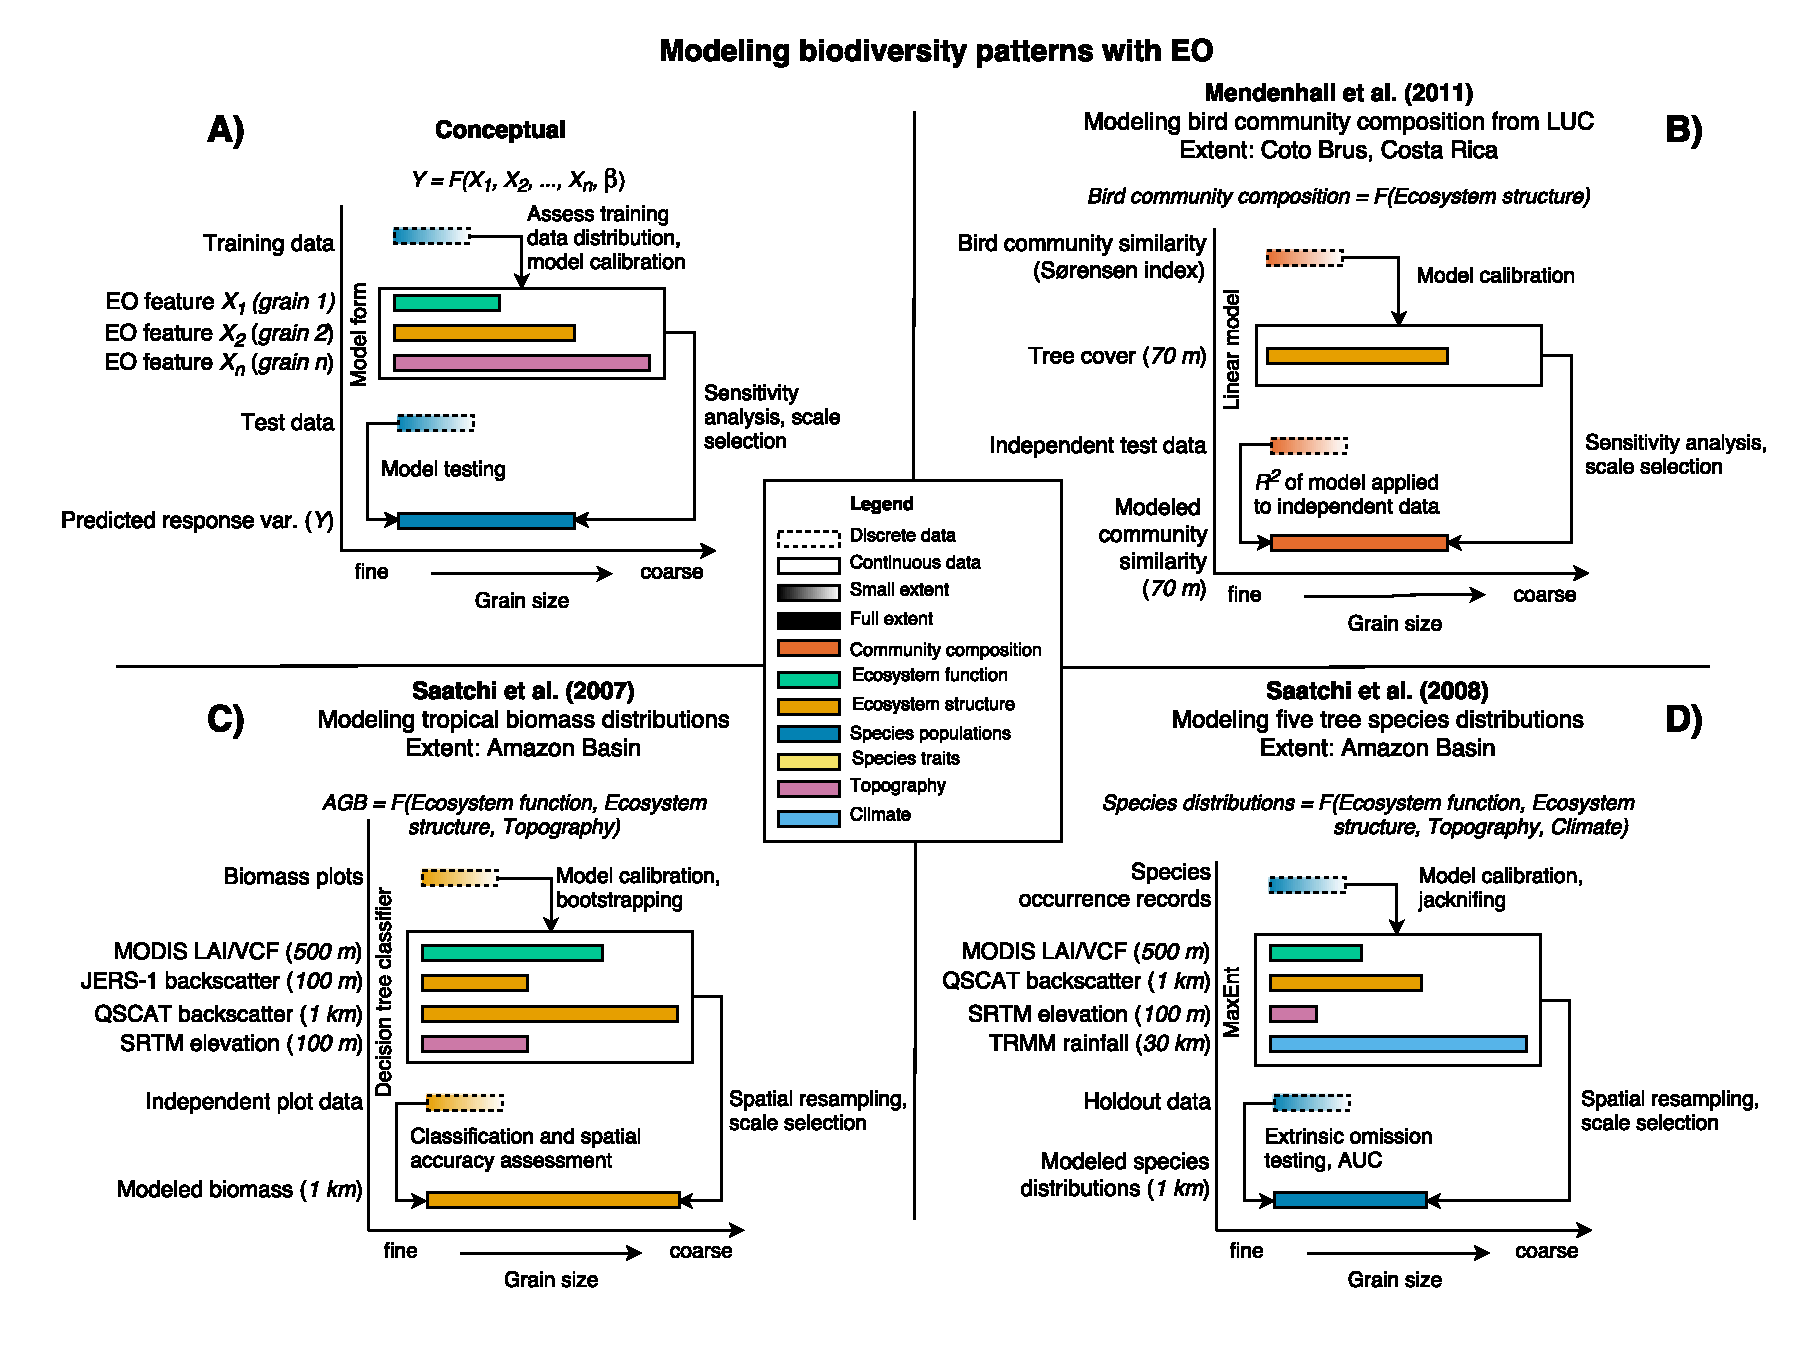
\includegraphics[width=\textwidth]{ch1-modeling}
\centering
\caption[Conceptual synthesis of how biodiversity patterns have been modelled using EO data at a single spatial scale.]{Biodiversity patterns are often modelled using EO data at a single spatial scale. (a) Conceptual model of how EO have been used to predict biodiversity patterns using supervised modelling approaches. (b) \cite{Mendenhall2011-mu} modeled bird community similarity as a function of tree cover across Coto Brus, Costa Rica. (c) \cite{Saatchi2007-sc} modeled aboveground biomass distributions across Amazonia. (d) \cite{Saatchi2008-jq} modeled tree species distributions across Amazonia.}
\label{fig:modeling}
\end{figure}

\subsection{Modeling Biodiversity Patterns}

Biodiversity patterns that are difficult to measure directly with EO are often modelled as a function of environmental features (Fig. \ref{fig:modeling}). There are many approaches to modelling biodiversity patterns with EO, including models of species‐scale (Fig. \ref{fig:modeling}d) \cite{Saatchi2008-jq}, community‐scale (Fig. \ref{fig:modeling}b) \cite{Mendenhall2011-mu} and ecosystem‐scale biodiversity patterns (Fig. \ref{fig:modeling}c) \cite{Saatchi2007-sc}. These approaches typically resample all data layers to a uniform grain size and extent, occasionally after multi‐scale sensitivity analysis \cite{mcgarigal2016multi}. Here I briefly discuss models of individual species distributions \cite{Guisan2005-kg} and models of community‐scale patterns like $\alpha$- and $\beta$-diversity \cite{Rocchini2007-ew}. These modelling methods have been reviewed elsewhere \cite{Gillespie2008-gi, Rocchini2010-pe, Pettorelli2014-pn}, but this section reviews role of scale in these approaches.

Species distribution models (SDMs) predict species geographical distributions across an extent as a function of environmental features that constrain niche use and niche availability \cite{Soberon2005-nz}. There have been many discussions on the importance of feature selection in SDM \cite{Booth2014-le, Brandt2017-ze, Fourcade2018-ws}, but some key reviews have emphasised that scale selection can play a similarly important role \cite{mayor2009habitat,mcgarigal2016multi}. Even so, studies addressing scale directly have found equivocal results. For example \cite{Guisan2007-zu} modelled bird and plant distributions at multiple grain sizes, finding only small decreases in model accuracy at coarser grain sizes on average. Disaggregating these results by taxon, however, revealed significant decreases in accuracy at coarser grains for all plants, but only some birds. In addition, species with the least training data saw the largest decreases in accuracy. \cite{Seo2009-ms} further explored these patterns in nine plant species, comparing both model accuracy and the spatial patterns of distributions. They found model accuracy decreased consistently at coarser grain sizes, and that these decreases were species‐specific. They also found significant spatial disagreement between models of varying grain size for each species, which could have major consequences for spatial conservation planning \cite{faleiro2013defining}.

There are two principal approaches to modelling community‐scale patterns with EO. First is to predict the distributions of all species in a community, then overlay these outputs to estimate community composition (i.e. stacked SDMs; \cite{Thuiller2009-ou,Calabrese2014-ct}. Second is to model community diversity metrics via regression \cite{Gillespie2008-gi, Saatchi2008-jq}. As above, the role of scale in these approaches has been equivocal. For example \cite{Thuiller2015-mn} modelled multiple plant community diversity metrics in the French Alps using a stacked‐SDM approach at varying grain sizes. They found that estimates of functional diversity, phylogenetic diversity and species richness all varied independently with changes in grain size. Functional diversity was best predicted at the finest grain size (250 m), whereas phylogenetic diversity and species richness were best predicted at coarser grain sizes (1000 m), suggesting scale dependence at the community scale is often process specific.

Assessing scale dependence in regression approaches has been done by comparing species richness predictions across multiple sensors. For example \cite{Nagendra2010-cc} modelled plant species richness using features from a fine grain, low fidelity sensor (IKONOS) and a moderate grain, high fidelity sensor (Landsat). Since community diversity metrics assess within‐ and between‐grain variation, one may expect that fine‐grain EO better predict these patterns. On the other hand, high fidelity measurements may better discriminate the between‐grain variation in environmental features that predict spatial turnover in communities. \cite{Nagendra2010-cc} found that, despite the coarser grain size, Landsat‐based models better predicted plot‐level species richness. Though the IKONOS data matched the grain size of the field plots, they failed to meaningfully discriminate the spatial variation in environmental features that predicted spatial richness patterns. Further disentangling the effects of sensor fidelity from variations in measurement scales will help discriminate sensor dependence from scale dependence in modelling other biodiversity patterns.

\subsection{Linking Measurements and Models}

EO measurements and models of biodiversity patterns are tightly connected. They are both subject to pattern‐specific scale dependencies, and multi‐scale comparisons or sensitivity analyses are essential for quantifying and understanding these dependencies. Furthermore, when EO measurements are the features used to model biodiversity patterns, scale‐dependent measurement variation becomes embedded within the models. This might obfuscate process‐driven scale dependence for variation driven by changing measurement scales. Constraining scale‐dependent variation in EO measurements of biodiversity patterns, and disentangling this variation from variation driven by sensor fidelity, will be key for reducing uncertainties in multi‐scale modelling efforts. In the following section I review some other challenges linking measurements and models of biodiversity patterns, and opportunities for multi‐scale analyses to address these challenges.

\section{Translating Biodiversity Patterns Across Scales}

One central challenge linking field and EO data is overcoming scale mismatches. These mismatches occur where response and feature data are sampled at disparate and irreconcilable scales. The size of field plots (i.e., the response data) are often much smaller than the grain size of EO sensors (i.e., the feature data), which can obscure key patterns and processes operating between these scales. For example \cite{Cleveland2015-zt} modelled spatial patterns of net primary productivity across the Amazon basin using three models at three scales: from plot data upscaled to the study extent ($0.1\, ha$ grain size), from MODIS data collected across the full extent ($1\, km^2$ grain size) and from a community land model ($12,500\, km^2$ grain size). These methods calculated the same average net primary productivity across the Amazon, indicating a potential convergence of the processes driving forest productivity. However, results from the finer‐scale methods were shown to be spatially independent from the others, indicating that they converged on the same average results for different reasons. In this case, comparing multiple models at mismatched scales that calculated the same result can make it difficult to disaggregate the role of process from the role of scale in understanding spatial patterns of productivity.

One key challenge in translating patterns across mismatched scales is capturing the dynamics of intermediate‐scale biodiversity patterns that are poorly characterised by field data. These patterns are too rare to be characterised by a small number of field plots, and are often difficult to reliably measure with coarse grained EO. For example, \cite{Fisher2008-sm} and \cite{Chambers2009-bl} identified that tree falls patterns, which tend to be both rare and spatially clustered, are underrepresented in field plots in the Amazon. Their analyses demonstrated that efforts to model related patterns using just field data (e.g., carbon sequestration) would necessarily underestimate feedbacks from these intermediate‐scale disturbances. Furthermore, \cite{Marvin2014-ms} quantified these mismatches using airborne lidar data, finding between 44 and 85 field plots per forest type would be required to characterise mean, community‐scale carbon and disturbance dynamics. Together, these results suggest that field measurements should be greatly expanded, or novel data should be used to characterise intermediate‐scale patterns in order to translate patterns across scales.

The challenges presented by scale mismatches can be framed by two tenets of the problem of pattern and scale: that multiple ecological processes can drive biodiversity patterns, and that there is rarely a single scale that best identifies how specific processes drive patterns \cite{Wiens1989-yi,Levin1992-ga}. These tenets suggest that multi‐scale analyses, which capture the intermediate‐scale patterns obscured between fine and coarse grain patterns, could improve empirical approaches to mapping biodiversity patterns with EO. Iteratively modelling patterns with multi‐scale EO has been used to map a range of biodiversity patterns at moderate grain sizes across large extents, and presents an actionable approach to overcoming some of the challenges presented by scale mismatches.

\subsection{Multi-scale Modeling}

\begin{figure}[!ht]
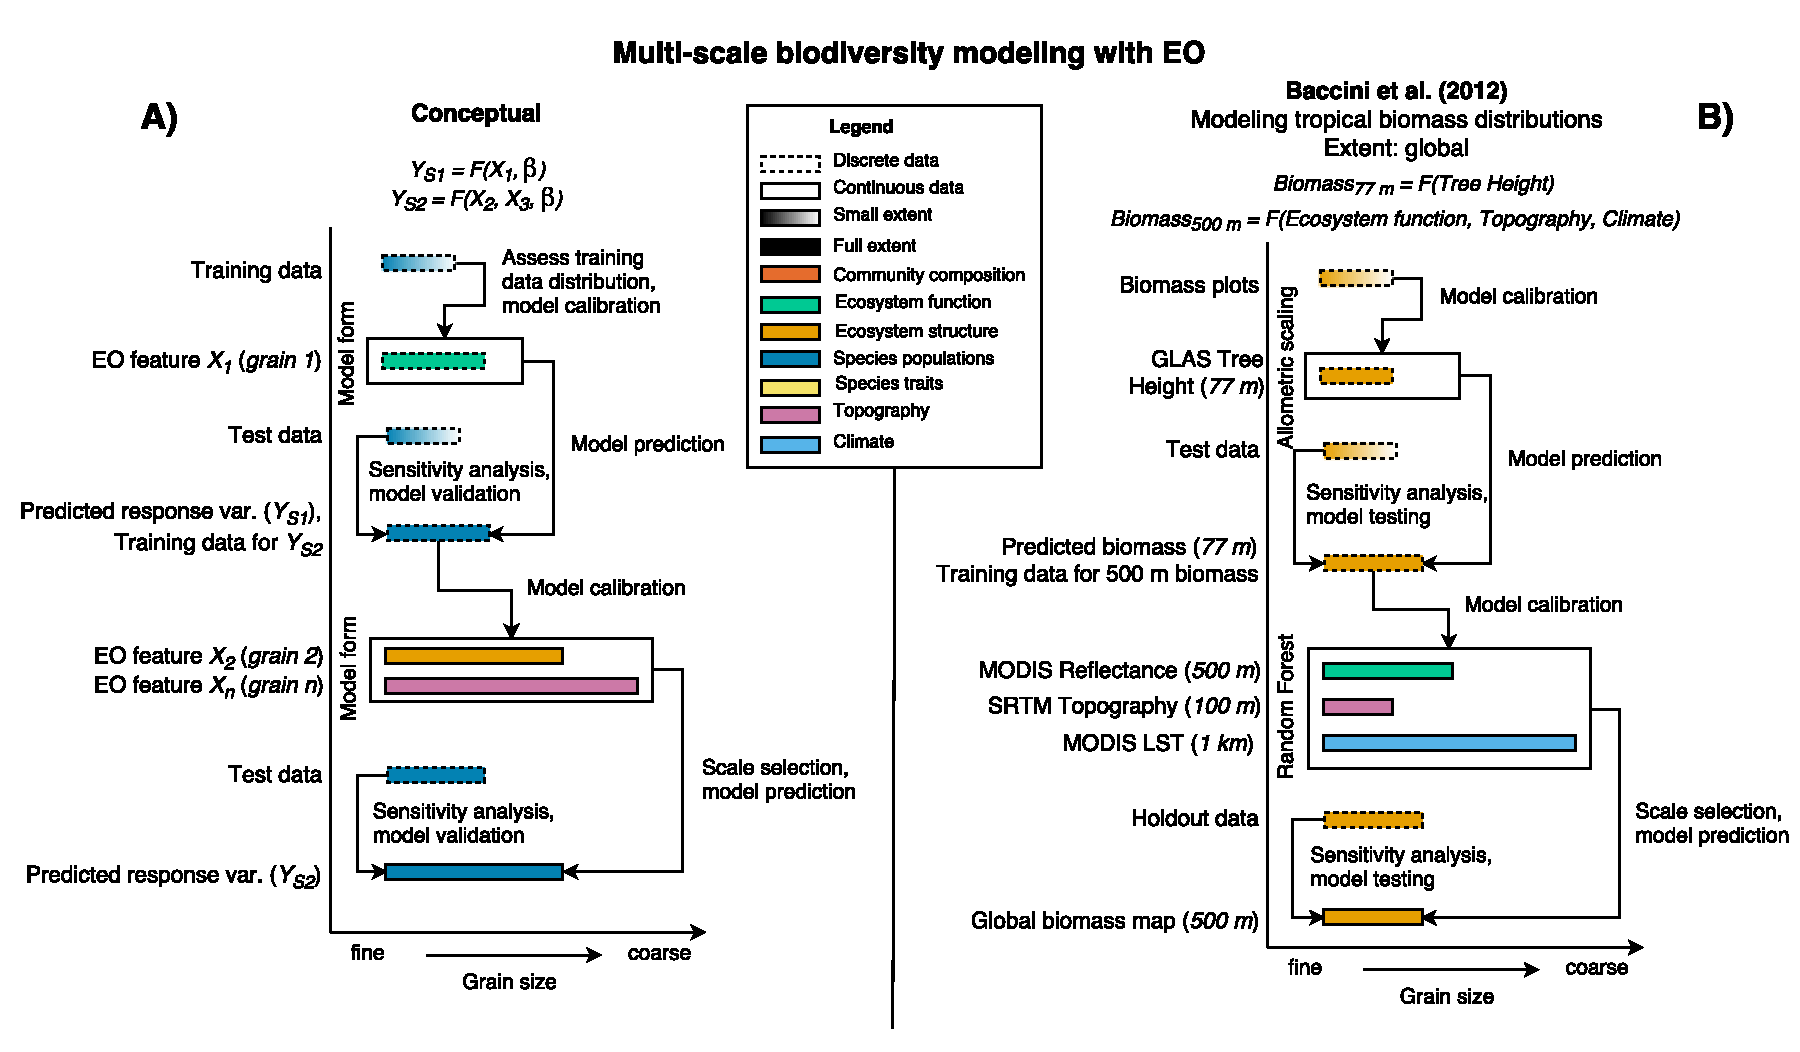
\includegraphics[width=\textwidth]{ch1-multiscale-modeling}
\centering
\caption[Conceptual synthesis of how biodiversity patterns have been modelled using EO data at multiple spatial scales.]{Leveraging coincident data from multiple sensors in a multi-scale framework provides opportunities to translate fine-scale biodiversity patterns across scales. (a) Conceptual model of how EO data have been used to predict biodiversity patterns using a multi‐scale modelling approach. (b) An example from \cite{Baccini2012-ow} demonstrating the multi‐scale modelling approach for predicting tropical biomass globally.}
\label{fig:multiscale-modeling}
\end{figure}

Multi‐scale models attempt to obviate scale mismatches through iteratively modelling patterns at varying grain sizes (Fig. \ref{fig:multiscale-modeling}a). One key innovation of the multi‐scale modelling approach was to leverage intermediate‐scale data sources that capture the extent‐wide variation in EO features, which is difficult to cover with field plots alone. For example, \cite{Baccini2012-ow} developed a benchmark map of pantropical aboveground biomass using a multi‐scale model, a network of field plots, discrete spaceborne lidar data ($4,900\, m^2$) and continuous, coarse grain EO ($0.25\, km^2$; Fig. \ref{fig:multiscale-modeling}b). First, they calibrated an allometric model using biomass plots coincident with lidar‐derived tree height data \textit{sensu} \cite{Chave2005-rs}. Next, they applied this model to all tree height measurements, creating a discrete, global biomass map. Finally, they modelled biomass continuously using a regression tree model, with lidar‐derived biomass as the response and EO data on climate, topography and ecosystem function as the environmental features. Their final map of aboveground biomass served as a benchmark for global carbon monitoring \cite{Ciais2014-rb}.

Multi‐scale models have also been used to monitor temporal changes using intermediate‐scale EO, overcoming some of the challenges highlighted by \cite{Fisher2008-sm} and \cite{Marvin2014-ms}. For example, \cite{Baccini2017-zk} assessed temporal patterns of change in aboveground biomass using EO measurements of forest growth, disturbance and deforestation. Intermediate‐scale disturbance measurements were essential for capturing the magnitude of change: their results revealed that disturbance accounts for nearly 70\% of forest emissions, and that the Earth's tropical forests are now a net source of carbon to the atmosphere. Considering how little is known about the rate, magnitude and direction of global biodiversity change \cite{Pereira2012-vm,mcgill2015fifteen}, I expect these multi‐scale analyses will prove essential for settling debates over other key knowledge gaps \cite{vellend2013global, Gonzalez2016-gh}. These analyses have also proven useful for mapping patterns that have been difficult to directly measure with publicly-accessible EO data: species traits.

\subsection{Mapping Plant Functional Traits}

Measuring species traits as a complement to species counts has become a priority for biodiversity science. Traits have been touted as a link between applied and theoretical biodiversity research and as a means to better represent ecosystem function in Earth systems models \cite{Shipley2006-lt,Jetz2016-bx,Funk2017-io}. Plant functional traits (PFTs) are one subset of species traits that can be mapped using EO, specifically by imaging spectroscopy \cite{Kokaly2009-xk}. One key benefit of measuring PFTs with EO is that they can be mapped without having to identify and characterise every species \textit{a priori}; capturing the range and variation in traits is often more important. The prospective launches of spaceborne imaging spectrometers, such as EnMAP, PRISMA and HISUI, are currently touted as the best bet for mapping PFTs globally \cite{Stuffler2007-ie, Galeazzi2008-lc, Matsunaga2011-ba}. Simulations from preparatory campaigns have found mixed results, however. For example, \cite{Bachmann2015-tt} demonstrated that the moderate fidelity of these sensors should lead to high variation in surface reflectance measurements (the basis for measuring PFTs). Furthermore, the moderate grain size of these sensors (30 m) has been shown to significantly reduce classification accuracy compared to fine‐grain measurements in other contexts \cite{Kruse2011-ck}. This decrease in accuracy is expected to be exacerbated for PFTs since canopy structure, not trait variation, drives the majority of reflectance signal at moderate grain sizes \cite{Yao2015-dp}. Combined, these sensor- and scale-dependent challenges spell major trouble for trait-based species mapping. This approach is predicated on the basis that differences in traits between species arise as a function of interpsecific niche partitioning and intraspecific niche conservation. That is, traits are typically conserved within a species and vary between species along axes of e.g. the plant economics spectrum \cite{Wright2004-md}. Tracking these patterns with EO could be for naught if intraspecific measurement variance is greater than the variance in interspecific measurements.

The implication is that spaceborne trait measurements may not yet provide a panacea for large-scale species mapping. Fortunately, airborne imaging spectrometers can measure species traits at the scales of individual organisms, and these measurements can be combined with other EO to model PFT distributions over large extents (Fig. \ref{fig:multiscale-modeling}a), as \cite{Asner2016-qd} demonstrated with a multi‐scale modelling approach to map PFTs across the Peruvian Amazon. First they measured PFTs for all canopy trees in a network of field plots, capturing the physiological range of each trait. Next they trained regression models using each trait as the response variable, and the imaging spectroscopy data as features. These trait models were then applied to all airborne data, which were collected across gradients of elevation, geology and forest type. Finally, they modelled these traits continuously using the airborne‐scale trait maps as the responses, and satellite measurements of ecosystem structure, ecosystem function, climate and topography as features. Since these traits vary widely within plots, and more so across the full study extent, the airborne‐scale trait maps were a representative sample of local‐scale trait variation across this high diversity region. The intermediate‐scale maps provided more data to train the satellite‐based models and, aggregated to the grain size of the satellite data, obviated problems of sampling effort and scale mismatch.

Applying these multi‐scale modelling approaches could enable monitoring similar biodiversity patterns that have otherwise proven difficult to map over large extents. Though access to intermediate‐scale data has been historically limited, it should increase with the launch of novel fine‐grain sensors \cite{Malenovsky2012-nv}. Monitoring intermediate‐scale patterns could be further bolstered by expanding the scope of airborne mapping by groups like NEON's Airborne Operations Platform \cite{Keller2008-dl}, DLR's Optical Airborne Remote Sensing platform (OpAiRS; \cite{Baumgartner2012-sg, Leutner2012-uc}, or the Carnegie Airborne Observatory (CAO; \cite{Asner2012-qs}). Linking field, airborne and spaceborne measurements could be used to map fine‐scale patterns like species traits across large extents, generate intermediate‐scale data to train and test satellite measurements, and link the distributions of community and ecosystem‐scale patterns to species identities \cite{Clark2005-kr, Baldeck2015-jd}. Furthermore, implementing large‐scale airborne mapping efforts could be done at a fraction of the price of building and launching a satellite \cite{Mascaro2014-js}.

\section{Frontiers in Monitoring Biodiversity Change with EO}

Global biodiversity monitoring systems hold great promise for advancing biodiversity science and conservation. These systems could be designed to forecast the rate, magnitude and geography of biodiversity change, identifying opportunities to mitigate human impacts on biological communities. EO can support monitoring systems by providing consistent and repeat assessments of biodiversity change; a unique global perspective of our changing biosphere. Applying concepts of pattern and scale in ecology to EO could link these fields in support of this vision. However, \cite{estes2018spatial} found there is currently little overlap in the ecology literature between studies analysing field data and studies analysing EO data, highlighting the wide gap between these communities. And the problems presented by scaling dynamics (e.g. scale mismatches) have helped frame EO science as distinct from ecology, as subject to different rules and standards. Developing an ecologically based framework for monitoring biodiversity change with EO will require overcoming this distinction.

There are several key similarities between field and EO data: changing their grain size or extent fundamentally alters within and between‐grain variation, there is rarely a single scale at which any pattern should be examined, and aggregating measurements to discrete domains of scale can constrain nonlinear responses to change. These similarities frame EO as an extension of field data; their differences are more in scale than they are in kind. Multi‐scale analyses linking field and EO data support this, emphasising that targeted field collections are essential for mapping biodiversity patterns that are difficult to measure independently with EO. In the context of biodiversity monitoring, field data play three key roles: training EO to map novel biodiversity patterns; developing and testing forecasts of biodiversity change, and constraining the extents to which we can generalise patterns of change.

\subsection{Ecologically Interpreting Sensor Data}

One key challenge in measuring biodiversity patterns with EO is converting at‐sensor measurements into biologically meaningful metrics of change (e.g. from at‐sensor radiance to percent tree cover). This is often done empirically via calibration with field measurements. These calibrations require a lot of data; EO data dimensionality is often very high and the variation in biological communities that drives measurement variance is similarly high. However, it is difficult for any one research group to independently collect the field data necessary to capture this variation. One way to overcome this challenge is to leverage open data. 

Access to open biodiversity data has increased dramatically over the past decade \cite{Kattge2011-tf, Jetz2012-mw, Metzger2013-mz, Culina2018-ih}, as has access to open EO data \cite{Nemani2011-ls, Irons2012-fm, Gorelick2017-nx}. And though there are known spatial, temporal and taxonomic gaps in open biodiversity data \cite{Beck2014-am, Geijzendorffer2016-xv}, extrapolating from incomplete measurements to fill these gaps is a key role for EO. Training global, multi‐scale EO models using centralised and curated field data could provide baseline estimates of spatial biodiversity patterns that have been otherwise difficult to characterise. These baselines could be tested independently by researchers with improved local data and local knowledge, identifying opportunities to improve regional and global models. These analyses could spur modelling and data collection efforts to fill gaps, and to develop better forecasting tools. These are urgently needed in ecology \cite{Dietze2018-eh}, and this theme is explored further in \textit{Chapter 3}.

\subsection{Reconciling Phenomenological and Process-based Models}

Another key role for field data is to develop and test predictive, process‐based models of temporal change. EO are uniquely suited for empirically monitoring change, especially for directly measurable patterns (e.g. disturbance) \cite{zhu2012continuous, cohen2016forest}. Yet forecasting change under conditions outside the range of historic variation (e.g. under novel climate and land‐use scenarios) remains a challenge for EO. Furthermore, temporal lags between local environmental change and other scales of change (e.g. for species or community‐scale patterns) can obfuscate efforts to identify the impacts of change \cite{essl2015delayed}. Developing process‐based models that couple temporal changes in EO to changes in other biodiversity patterns could address these issues \cite{korzukhin1996process,adams2013empirical}. 

While there are many process‐based EO models, and many process‐based biodiversity models, we now have the technical capacity to link and test them using open data at multiple scales, identifying consensus models and key data gaps. Coupling process‐based models with long‐term, regularly updated and globally consistent measurements of change from EO could be used to develop early warning systems for identifying where species, communities and ecosystems will respond to change in novel ways, and may identify opportunities for science‐driven mitigation (Daily 1999; Scholes et al . 2008). This theme is explored further in \textit{Chapter 4}.

\subsection{Bounding the Domains of Scale}

Finally, field data are key for constraining how we generalise EO measurements and models of biodiversity change. One advantage of monitoring change with EO is that measurements are globally consistent; tree cover change can be mapped across tropical, temperate and boreal forests \cite{Hansen2013-oz, Sexton2013-rk}. This enables other models of change that use tree cover data as features to be applied globally, such as the models of community composition in \cite{Mendenhall2016-xz}. This would be imprecise, however; the relationships between tree cover and community composition in tropical countrysides may not apply to timber plantations. In other words, this model is not stationary; the relationships between feature and response variables can change across the extent of the data \cite{Hawkins2012-gu}. The regions over which these relationships are stationary can be considered domains of scale, constraining the extents to which a model can generalise. It is currently difficult to identify these domains of scale with EO alone. Several algorithms can be employed to automate this task for EO (e.g. segmentation, clustering), but field data are key for interpreting and constraining these extents to biologically meaningful domains, and for testing their accuracy. Linking field and EO data to identify these domains of scale will be central to ecologically translating knowledge of local biodiversity patterns to regional and global scales.

\subsection{Conclusion}

After decades of work from biodiversity scientists, EO scientists and conservation groups, the stage is now set to establish ambitious, science‐driven biodiversity monitoring systems. Consistent, repeat and globally available EO will play a key role in these systems. Scale is a central and unifying concept for biodiversity and EO sciences, and monitoring change with EO should be based on the principles and ecology of scale. Global biodiversity monitoring promises to expand our understanding of Earth's species, communities and ecosystems and, with luck, could help us discover the wisdom necessary to conserve them.

\clearpage